\documentclass[tikz,border=8pt]{standalone}
\usepackage{amsmath,amssymb,bm}
\usepackage{sansmath}
\usepackage{tikz}
\usetikzlibrary{arrows.meta,calc}
\usepackage{pgfplots}
\pgfplotsset{compat=1.16}
\usepgfplotslibrary{groupplots}
\definecolor{cteal}{HTML}{2F5D62}\definecolor{cred}{HTML}{A44A3F}\definecolor{cochre}{HTML}{B08A45}
\definecolor{cgray}{HTML}{666360}\definecolor{clgray}{HTML}{9A9791}\definecolor{csage}{HTML}{7D9D8C}
\definecolor{cpurple}{HTML}{7A5B78}\definecolor{cdark}{HTML}{3B3A38}\definecolor{cmid}{HTML}{8E8B85}\definecolor{cpaper}{HTML}{F6F4F0}
\pgfplotsset{paper/.style={font=\sffamily\sansmath\scriptsize, axis line style={black!65,line width=0.4pt},
  tick style={black!65,line width=0.4pt}, tick align=outside, major tick length=2pt,
  axis x line*=bottom, axis y line*=left, grid style={line width=0.3pt,black!10},
  legend style={draw=none,fill=none,font=\sffamily\sansmath\scriptsize}, legend cell align=left,
  title style={font=\sffamily\sansmath\scriptsize,at={(0,1)},anchor=south west,yshift=3pt,xshift=-2pt},
  label style={font=\sffamily\sansmath\scriptsize}, ticklabel style={font=\sffamily\sansmath\scriptsize},
  yticklabel style={font=\sffamily\sansmath\scriptsize}, xticklabel style={font=\sffamily\sansmath\scriptsize}}}


\newcommand{\logit}{\operatorname{logit}}\newcommand{\expit}{\operatorname{expit}}
\begin{document}
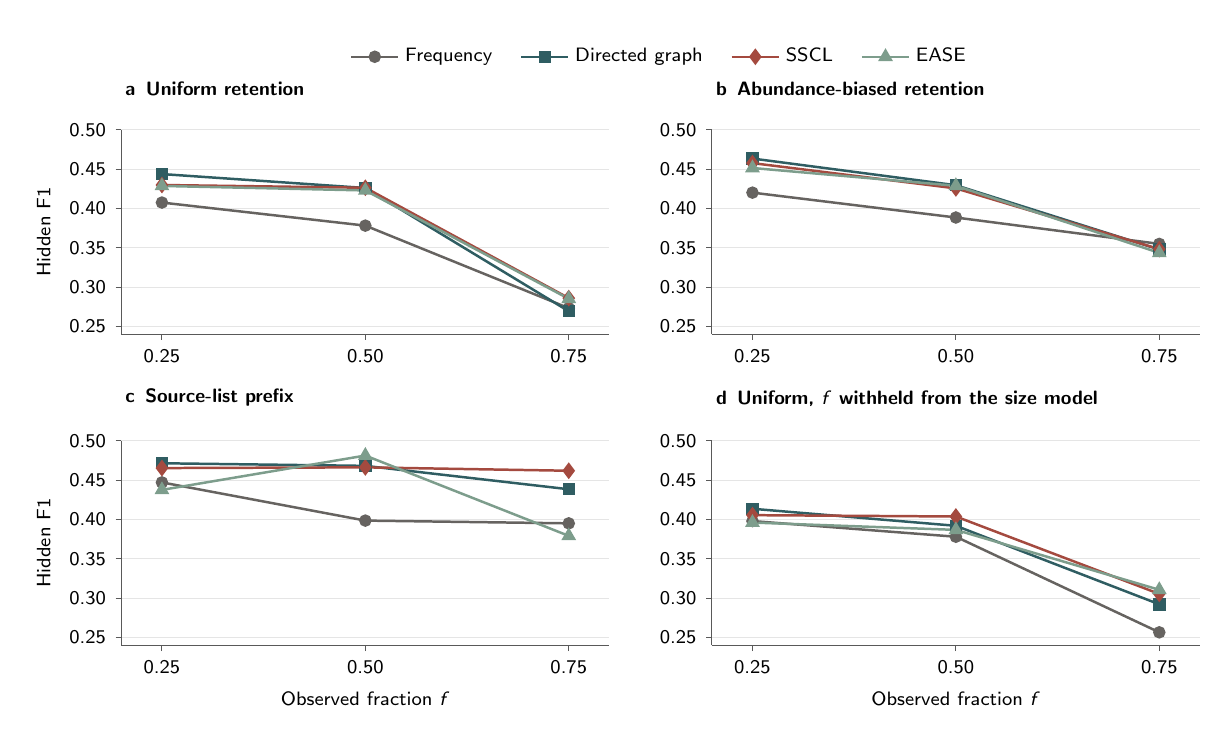
\begin{tikzpicture}
\begin{groupplot}[paper, group style={group size=2 by 2, horizontal sep=1.3cm, vertical sep=1.35cm,
     xlabels at=edge bottom, ylabels at=edge left},
  scale only axis, width=6.2cm, height=2.6cm, xmin=0.2, xmax=0.8, ymin=0.24, ymax=0.50,
  xtick={0.25,0.5,0.75}, xticklabels={0.25,0.50,0.75}, ytick={0.25,0.30,0.35,0.40,0.45,0.50},
  yticklabel style={/pgf/number format/fixed,/pgf/number format/precision=2,/pgf/number format/fixed zerofill},
  ymajorgrids, xlabel={Observed fraction $f$}, ylabel={Hidden F1},
  every axis plot/.append style={line width=0.9pt,mark size=1.8pt}]
\nextgroupplot[title={\textbf{a}\enspace\textbf{Uniform retention}},
  legend to name=fivelegend, legend columns=4, legend style={/tikz/every even column/.append style={column sep=8pt}}]
\addplot[color=cgray,mark=*] coordinates {(0.25,0.4075) (0.5,0.3782) (0.75,0.2734)};
\addplot[color=cteal,mark=square*] coordinates {(0.25,0.4437) (0.5,0.4260) (0.75,0.2695)};
\addplot[color=cred,mark=diamond*,mark size=2.3pt] coordinates {(0.25,0.4298) (0.5,0.4263) (0.75,0.2861)};
\addplot[color=csage,mark=triangle*,mark size=2.2pt] coordinates {(0.25,0.4286) (0.5,0.4229) (0.75,0.2853)};
\legend{Frequency,Directed graph,SSCL,EASE}
\nextgroupplot[title={\textbf{b}\enspace\textbf{Abundance-biased retention}}]
\addplot[color=cgray,mark=*] coordinates {(0.25,0.4201) (0.5,0.3885) (0.75,0.3550)};
\addplot[color=cteal,mark=square*] coordinates {(0.25,0.4634) (0.5,0.4295) (0.75,0.3478)};
\addplot[color=cred,mark=diamond*,mark size=2.3pt] coordinates {(0.25,0.4576) (0.5,0.4255) (0.75,0.3484)};
\addplot[color=csage,mark=triangle*,mark size=2.2pt] coordinates {(0.25,0.4514) (0.5,0.4288) (0.75,0.3436)};
\nextgroupplot[title={\textbf{c}\enspace\textbf{Source-list prefix}}]
\addplot[color=cgray,mark=*] coordinates {(0.25,0.4471) (0.5,0.3986) (0.75,0.3951)};
\addplot[color=cteal,mark=square*] coordinates {(0.25,0.4714) (0.5,0.4681) (0.75,0.4384)};
\addplot[color=cred,mark=diamond*,mark size=2.3pt] coordinates {(0.25,0.4653) (0.5,0.4662) (0.75,0.4619)};
\addplot[color=csage,mark=triangle*,mark size=2.2pt] coordinates {(0.25,0.4376) (0.5,0.4812) (0.75,0.3792)};
\nextgroupplot[title={\textbf{d}\enspace\textbf{Uniform, $f$ withheld from the size model}}]
\addplot[color=cgray,mark=*] coordinates {(0.25,0.3980) (0.5,0.3781) (0.75,0.2567)};
\addplot[color=cteal,mark=square*] coordinates {(0.25,0.4136) (0.5,0.3920) (0.75,0.2923)};
\addplot[color=cred,mark=diamond*,mark size=2.3pt] coordinates {(0.25,0.4055) (0.5,0.4038) (0.75,0.3055)};
\addplot[color=csage,mark=triangle*,mark size=2.2pt] coordinates {(0.25,0.3961) (0.5,0.3868) (0.75,0.3107)};
\end{groupplot}
\node[anchor=south] at ($(group c1r1.north)!0.5!(group c2r1.north)+(0,0.55cm)$) {\pgfplotslegendfromname{fivelegend}};
\end{tikzpicture}
\end{document}
